
% Documentclass with option with one column text layout
\documentclass[a4paper,twoside,11pt]{scrartcl}

% Documentclass with option to have two column text layout
%\documentclass[a4paper,twocolumn,11pt]{scrartcl}

% Package for generated dummy text
\usepackage{lipsum}

% Make table of contents entries links to sections in document clickable.
\usepackage[pdfborder=0]{hyperref}

% Make includegraphics available
\usepackage{graphicx}

% Include \section{} in the table of contents
\KOMAoption{toc}{sectionentrywithdots}

\title{Title of our work}

\author{
  Stefan Koenen, M.Sc. \\
  Faculty of Communication and Environment \\
  Ambient Intelligent Systems \\
  University of applied sciences Rhein-Waal \\
  stefan.koenen@hochschule-rhein-waal.de \\

\and

  Prof. Dr.-Ing. Christian Ressel \\
  Faculty of Communication and Environment \\
  Chair of Ambient Intelligent Systems \\
  University of applied sciences Rhein-Waal \\
  christian.ressel@hochschule-rhein-waal.de
}

%\date{2020-11-09}
\date{~}

% Set space between paragraphs
% em is measure of text height
\setlength{\parskip}{2em}

% Modify the indentation of the first sentence in a paragraph
\setlength{\parindent}{3em}
% To disable indent here use 0pt as value

\begin{document}

\pagenumbering{gobble} % No page numbers from here on

\maketitle

\clearpage

\pagenumbering{roman} % Page numbers are I II III IV V VI VII VIII IX X XI
\tableofcontents

% Print index of tables
\listoftables

% Print index of figures
\listoffigures

\clearpage
\pagenumbering{arabic}

%\section{Abstract}

Just some abstract text.

\section{Introduction}

This is just some introduction text for \LaTeX.
This is another sentence in this same paragraph.
Lets make some more sentences.
What should we write as sentences?
Maybe we should write about sentences?
Haha, no we don't do it.

Another paragraph.

This is another paragraph.

\lipsum{1-8}

\subsection{State of Art}

Just some state of art.



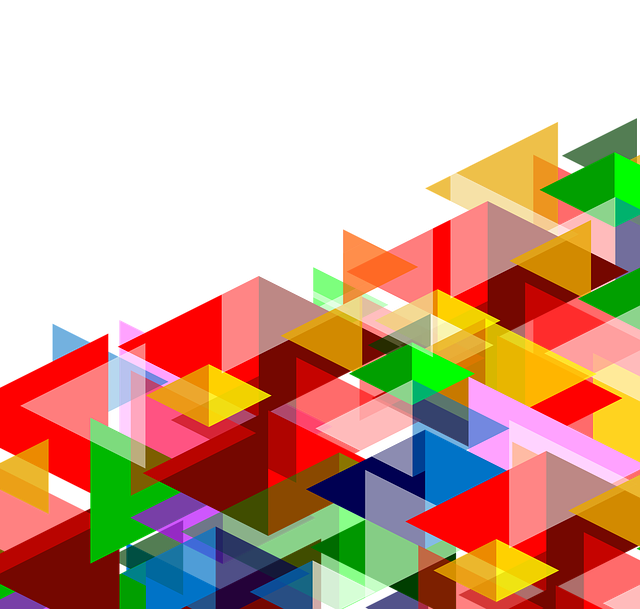
\includegraphics[scale=0.5]{../graphics}

%\begin{tabular}{ | l | r | c | }
%\end{tabular}

In the following we assume that 
$ a_x = x * 2 $
is always valid.

\begin{equation}
  y_{x*2 + sqrt{4*y}} = 10
\end{equation}


\end{document}
